\chapter{Background}
\blindtext

Studies show that the world is round\cite{Einstein1905}. See Fig.~\ref{fig:travelling plane wave} for more information.

\begin{figure}
    \centering
    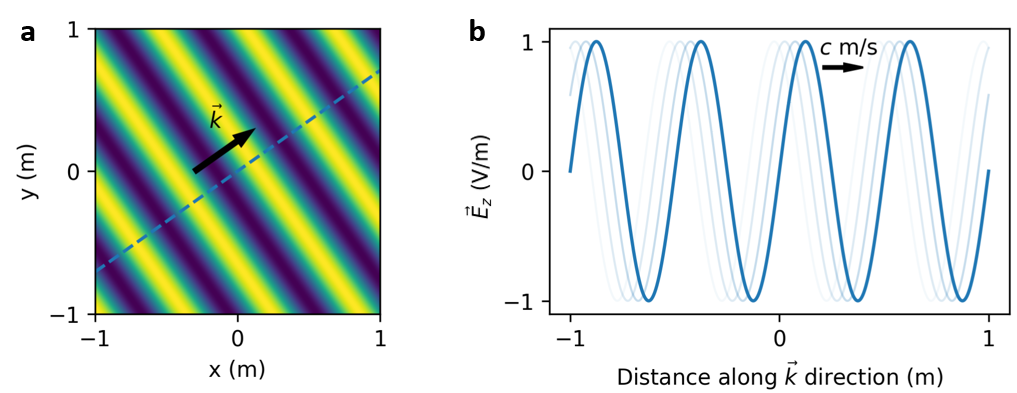
\includegraphics[width=\linewidth]{chap2/images/travelling plane wave.png}
    \caption{The classical travelling plane wave, the basis for field quantisation, is described by a wave vector $\vec{k}$ pointing in some direction in 3D space and having wavelength $\lambda = 2 \pi / |\vec{k}|$. a) A depiction of the field amplitude $|\vec{E}|$ for a given plane wave linearly polarised along $\vec{z}$ at a snapshot in time. b) The amplitude oscillates along the dashed line in (a). The wavefronts propagate along the $\vec{k}$ direction over time at speed $c$.}
    \label{fig:travelling plane wave}
\end{figure}

\section{Subsections and Subsubsections}

This is a section.

\subsection{A Subsection}

This is a subsection.

\subsubsection{A Subsubsection}

This is a subsubsection.

\section{Footnotes}

Some text with a footnote, if an online link remember to add \textit{Last Accessed}.\footnote{Some footnote text.}

\section{Equations}

The following is the most beautiful equation in maths, Euler's Identity (Equation~\ref{eq:euleridentity}).

\begin{equation}\label{eq:euleridentity}
	e^{i\pi}+1=0
\end{equation}

\blindtext

\section{Numbered Lists}

This is an example of a numbered list:

\begin{enumerate}
	\item This is my first point
	\item My second
	\item My third!
	\item And my fourth?
\end{enumerate}

\blindtext

\section{Bulleted Lists}

This is an example of a bulleted list:

\begin{itemize}
	\item This is my first point
	\item My second
	\item My third!
	\item And my fourth?
\end{itemize}



\section{Summary}
\blindtext